\documentclass{article}

% BASIC LIBRARIES
\usepackage[english]{babel}
\usepackage{graphicx}
\usepackage{siunitx}
\usepackage{amsmath}
\usepackage{physics}
\usepackage{subcaption}

% TIKZ LIBRARIES
\usepackage{tikz}
\usepackage[compat=1.1.0]{tikz-feynman}
\usepackage{pgfplots}
\pgfplotsset{width=10cm,compat=1.9}
\usepgfplotslibrary{external}
\usetikzlibrary{calc}

\begin{document}

\begin{figure}[htp]
\centering
\begin{minipage}{0.4\textwidth}
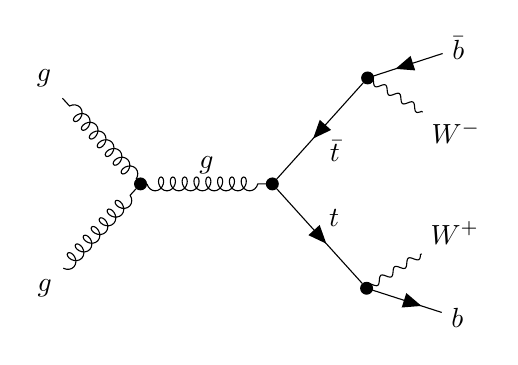
\begin{tikzpicture}
  \begin{feynman}[scale=1.1]
    \diagram[horizontal=a to b] 
     {
      i1 [particle=\(g\)] -- [gluon] a[dot,black] -- [gluon] i2 [particle=\(g\)],
      a -- [gluon, edge label=\(g\)] b[dot,black],
      f1 [particle=\(\bar{t}\), dot, black] -- [fermion, edge label=\(\bar{t}\)] b -- [fermion, edge label=\(t\)] f2  [particle=\(t\), dot, black],
     };
    \vertex at ($(b)!1!(f2)$) (p);
    \vertex at ($(p)!-1.2cm!80:(b)$) (r) {\(W^{+}\)};
    \draw [boson] (r) -- (p);
    
    \vertex at ($(b)!1!(f2)$) (p);
    \vertex at ($(p)!-1.1cm!30:(b)$) (r) {\(b\)};
    \draw [anti fermion] (r) -- (p);
    
    \vertex at ($(b)!1!(f1)$) (p);
    \vertex at ($(p)!-1.2cm!-80:(b)$) (r) {\(W^{-}\)};
    \draw [boson] (r) -- (p);
    
    \vertex at ($(b)!1!(f1)$) (p);
    \vertex at ($(p)!-1.1cm!-30:(b)$) (r) {\(\bar{b}\)};
    \draw [fermion] (r) -- (p);
  \end{feynman}
\end{tikzpicture}
\subcaption{Doubly-resonant diagram.}
\end{minipage}
\hspace{12mm}
\begin{minipage}{0.47\textwidth}
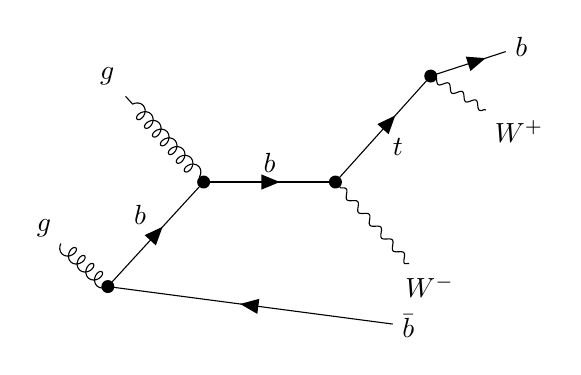
\begin{tikzpicture}
  \begin{feynman}[scale=1.1]
    \diagram[horizontal=a to b] 
     {
      i1 [dot,black]
        -- [fermion, edge label=\(b\)] a[dot,black]
        -- [gluon] i2[particle=\(g\)],
      a -- [fermion, edge label=\(b\)] b[dot,black],
      f1 [particle=\(t\), dot, black]
        -- [anti fermion, edge label=\(t\)] b
        -- [boson] f2 [particle=\(W^{-}\)],
     };
    \vertex at ($(i1)!.0!(a)$) (p);
    \vertex at ($(p)!1cm!90:(a)$) (r) {\(g\)};
    \draw [gluon] (r) -- (p);
    
    \vertex at ($(i1)!.0!(a)$) (p);
    \vertex at ($(p)!-3.5cm!125:(a)$) (r) {\(\bar{b}\)};
    \draw [fermion] (r) -- (p);
    
    \vertex at ($(b)!1!(f1)$) (p);
    \vertex at ($(p)!-1.2cm!-80:(b)$) (r) {\(W^{+}\)};
    \draw [boson] (r) -- (p);
    
    \vertex at ($(b)!1!(f1)$) (p);
    \vertex at ($(p)!-1.1cm!-30:(b)$) (r) {\(b\)};
    \draw [anti fermion] (r) -- (p);
    
  \end{feynman}
\end{tikzpicture}
\vspace{-5.5mm}
\subcaption{Singly-resonant diagram.}
\end{minipage}
\end{figure}

\begin{figure}[h!]
\centering
\begin{minipage}{0.4\textwidth}
\centering
\feynmandiagram [scale=1.0][baseline=(d.base), horizontal=d to b]  {
  a -- [gluon] b [dot,black] -- [gluon] c,
  b -- [gluon] d,
 };
\subcaption{Triple-boson vertex.}
\end{minipage}
\hspace{15mm}
\begin{minipage}{0.4\textwidth}
\centering
  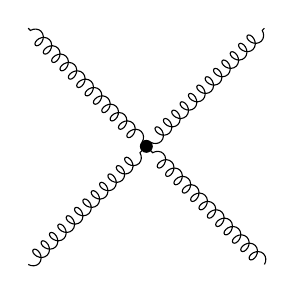
\begin{tikzpicture}
    \begin{feynman}[scale=0.75]
      \vertex (a) at (-2,-2);
      \vertex (b) at ( 2,-2);
      \vertex (c) at (-2, 2);
      \vertex (d) at ( 2, 2);
      \diagram* 
       {
        (a) -- [gluon] m [dot,black] -- [gluon] (c),
        (b) -- [gluon] m [dot,black] -- [gluon] (d),
       };
    \end{feynman}
  \end{tikzpicture}
  \vspace{0.25cm}
\subcaption{Tetra-boson vertex.}
\end{minipage}
\end{figure}

\begin{figure}[h!]
    \centering
    \begin{minipage}{0.4\textwidth}
    \centering
        \feynmandiagram [scale=1.95][inline=(d.base), horizontal=b to d] {
        a [particle=\(\alpha\)] -- [fermion] b [dot,black,label=180:\(- \dfrac{i g_s}{2} (\bm{\sigma}^i)_{\alpha\beta} \bm{\gamma}_{\mu}\)] -- [fermion] c [particle=\(\beta\)],
        b -- [gluon] d [particle=\(g\)],
        };
    \subcaption{Vertex factor of the interaction between nucleon and gauge field.}
    \end{minipage}
\hspace{15mm}
    \begin{minipage}{0.4\textwidth}
    \centering
        \feynmandiagram [scale=1.5][horizontal=a to b] {
        i1 [particle=\(\alpha\)] -- [fermion] a [dot,black] -- [fermion] i2 [particle=\(\beta\)],
        a -- [gluon, edge label=\(g\)] b [dot,black],
        f1 [particle=\(\delta\)] -- [anti fermion] b -- [anti fermion] f2 [particle=\(\gamma\)],
        };
    \subcaption{Nucleon-nucleon interaction.}
    \end{minipage}
\end{figure}
    
\begin{figure}[h!]
    \centering
    \begin{minipage}{0.4\textwidth}
    \centering
    \vspace{1.2cm}
        \feynmandiagram [scale=1.95][inline=(d.base), vertical=b to d] {
        a [particle=\(b\)] -- [blue, fermion] b [dot,black] -- [red, fermion] c [particle=\(r\)],
        b -- [gluon] d [particle=\(r \bar{b}\)],
        };
    \vspace{0.8cm}
    \subcaption{Vertex factor of the color interaction between quark and gluon.}
    \label{fig:color_vertex}
    \end{minipage}
\hspace{15mm}
    \begin{minipage}{0.4\textwidth}
    \centering
        \feynmandiagram [scale=1.5][vertical=a to b] {
        i1 [particle=\(r\)] -- [red,fermion] a -- [blue,fermion] i2 [particle=\(b\)],
        a -- [gluon, edge label=\(b\bar{r}\)] b,
        f1 [particle=\(r\)] -- [red, anti fermion] b -- [blue,anti fermion] f2 [particle=\(b\)],
        };
    \subcaption{Quark-quark color interaction: $qq^{'} \rightarrow q q^{'}$. The gluon carries the $b \bar{r}$ color.}
    \end{minipage}
\end{figure}

\begin{figure}[h!]
    \centering
    \begin{minipage}{0.4\textwidth}
    \centering
        \feynmandiagram [scale=1.3][layered layout, horizontal=b to c] {
        a -- [gluon] b [dot,black]
        -- [anti fermion, half left,edge label = $\bar{q}$] c [dot,black]
        -- [anti fermion, half left,edge label = $q$] b,
        c -- [gluon] d,
        };
    \subcaption{Quark loop radiation.}
    \end{minipage}
    \hspace{15mm}
    \begin{minipage}{0.4\textwidth}
    \centering
        \feynmandiagram [scale=1.3][layered layout, horizontal=b to c] {
        a -- [gluon] b [dot,black]
        -- [gluon, half left,edge label = $g$] c [dot,black]
        -- [gluon, half left,edge label = $g$] b,
        c -- [gluon] d,
        };
    \subcaption{Gluon loop radiation.}
    \end{minipage}
\end{figure}

\begin{figure}[h!]
\centering
\feynmandiagram [scale=1.7][layered layout, horizontal=a to b] {
    a [particle=\(n(d)\)] -- [fermion] b [dot,black] -- [fermion] f1 [particle=\(p(u)\)],
    b -- [boson, edge label'=\(W^{-}\)] c [dot,black],
    c -- [anti fermion] f2 [particle=\(\overline \nu_{e}\)],
    c -- [fermion] f3 [particle=\(e^{-}\)],
};
\caption*{Feynman representation of the $\beta$-decay of the neutron: $n \rightarrow p + e^{-} + \bar{\nu}_{e}$.}
\end{figure}

\begin{figure}[h!]
\centering
\begin{minipage}{0.4\textwidth}
\feynmandiagram [scale=2.15][inline=(d.base), vertical=b to d] {
    a [particle=\(f\)] -- [fermion] b [dot,black] -- [fermion] c [particle=\(f\)],
    b -- [boson] d [particle=\(Z\)],
    };
\subcaption{NC interaction vertex.}
\end{minipage}
\hspace{15mm}
\begin{minipage}{0.4\textwidth}
\feynmandiagram [scale=2.15][inline=(d.base), vertical=b to d] {
    a [particle=\(l^{-}\)] -- [fermion] b [dot,black] -- [fermion] c [particle=\(\nu_{l}\)],
    b -- [boson] d [particle=\(W\)],
    };
\subcaption{CC interaction vertex.}
\end{minipage} 
\end{figure}

\end{document}
